\documentclass[11pt,twosided]{report}

\usepackage[titletoc]{appendix} % for adding appendix to TOC
\usepackage{biblatex}  % reference management
\usepackage{geometry}  % better margins and margin control
\usepackage{graphicx}  % to include figures
% \usepackage{hyperref}  % internal and external links
\usepackage[utf8]{inputenc}  % support for non-ASCII characters
\usepackage{listings}  % typset code
\usepackage{outlines}  % easy nesting of lists
\usepackage{tabularx}  % more control over table column width
\usepackage{titlesec}  % customize chapter title 
\usepackage{upquote}  % prevent mishandling of single quotes in listings
\usepackage{xcolor}
\usepackage{pgfgantt}
\usepackage{amsmath}
\usepackage{rotating}
\usepackage[graphicx]{realboxes}
\usepackage{attachfile}

\hypersetup{
    colorlinks=true,
    linkcolor=blue,
    filecolor=blue,      
    urlcolor=blue,
    citecolor= blue,
    pdftitle={SRS - Team Prions}
    }


% \definecolor{barblue}{RGB}{153,204,254}
% \definecolor{groupblue}{RGB}{51,102,254}
% \definecolor{linkred}{RGB}{165,0,33}
% \renewcommand\sfdefault{phv}
% \renewcommand\mddefault{mc}
% \renewcommand\bfdefault{bc}
% \setganttlinklabel{s-s}{START-TO-START}
% \setganttlinklabel{f-s}{FINISH-TO-START}
% \setganttlinklabel{f-f}{FINISH-TO-FINISH}
% \sffamily

% \newgantttimeslotformat{stardate}{%
% \def\decomposestardate##1.##2\relax{%
% \def\stardateyear{##1}\def\stardateday{##2}%
% }%
% \decomposestardate#1\relax%
% \pgfcalendardatetojulian{\stardateyear-01-01}{#2}%
% \advance#2 by-1\relax%
% \advance#2 by\stardateday\relax%
% }


% TODO: Customize the appearance of hyperref links using \hypersetup
% See https://en.wikibooks.org/wiki/LaTeX/Hyperlinks#Customization

% Custom format of chapter title.
\titleformat{\chapter}[hang]{\bf\huge}{\thechapter.}{2pc}{}

% Separate folder for images named 'images'.
\graphicspath{ {images/} }

% Separate file for references
\addbibresource{references.bib}

% Replace with your title
\title{A Novel Approach to PPI Network Analysis}

% Allow recalling document title
% from https://tex.stackexchange.com/a/15806/44301
\makeatletter\let\Title\@title\makeatother  

\begin{document}

\begin{titlepage}
  
  \newgeometry{top=100pt,bottom=75pt}   
  \begin{center}
    \vfill
    \textbf{\Huge \Title}
    \bigskip

    {\large Kaavish Report\\
      presented to the academic faculty\\
      by\\\bigskip
      % replace with your name and HU ID
  \begin{minipage}{0.85\textwidth} % Type Team Members Details here
    \begin{center} \large
    Ali \textsc{Hamza}\\ (\href{mailto:ah05084@st.habib.edu.pk}{\texttt{ah05084@st.habib.edu.pk}}) \\
    Haris Karim \textsc{Ladhani}\\ (\href{mailto:hl04349@st.habib.edu.pk}{\texttt{hl04349@st.habib.edu.pk}})\\
    Maham Shoaib \textsc{Patel} \\ \href{mailto: (mp04911@st.habib.edu.pk)}{(\texttt{mp04911@st.habib.edu.pk})}\\
    Muhammad Usaid \textsc{Rehman} \\ (\href{mailto:mr04302@st.habib.edu.pk}{\texttt{mr04302@st.habib.edu.pk}}) \\
    \end{center}
\end{minipage}



    }\vfill
    
\includegraphics[width=.4\textwidth]{./HU_logo_new.png}\\
    {\large In partial fulfillment of the requirements for\\
      \textit{Bachelor of Science}\\
      Computer Science\\\medskip
      \textbf{Dhanani School of Science and Engineering}\\\medskip
      Habib University\\\smallskip
      Spring 2022
    }\\\vfill
    Copyright {\scriptsize \textcopyright} 2019 Habib University
  \end{center}
  \restoregeometry
\end{titlepage}

%%% Local Variables:
%%% mode: latex
%%% TeX-master: "report"
%%% End:
  % title page.
\thispagestyle{empty}
\centerline{\textbf{\LARGE \Title}}
\vfill

This Kaavish project was supervised by:\\\bigskip\\\bigskip\\\bigskip

% TODO: Use the appropriate table below depending on whether you have an external advisor. Comment out the unused table.

% If no external supervisor.
\hfill %
\begin{tabular}{l}
  \line(1,0){200}\\
  My Internal Supervisor \\ % Name of your CS supervisor
  Faculty of Computer Science\\
  Habib University
\end{tabular}\\\bigskip\bigskip

% % If external supervisor.
% \begin{tabularx}{\linewidth}{lXl}
%   \line(1,0){175} & & \line(1,0){175}\\  % Signatures.
%   My External Supervisor & & My Internal Supervisor \\ % Names of your supervisors
%   Designation & & Faculty of Computer Science\\  % External supervisor's role/job tile at their company.
%   Awesome Ltd. & & Habib University  % External supervisor's company.
% \end{tabularx}\\\bigskip\bigskip

Approved by the Faculty of Computer Science on \hrulefill.

%%% Local Variables:
%%% mode: latex
%%% TeX-master: "report"
%%% End:
  % approval page.

% \chapter*{Dedication}
% For ammi, abbu, and pappu.

% \chapter*{Acknowledgements}
% We want to thank the CS faculty and ...

% \chapter*{Abstract}
% Abstract goes here

% The following are automatically populated by LaTeX \chapter, \section and related, \figure, and \table.
\tableofcontents
% \listoffigures
% \listoftables

\chapter{Introduction}
\label{chap:intro}


\section{Problem Statement}

The protein-protein interaction (PPI) is a vastly studied area and thus there are various datasets and computational methods available to tackle the issue but these are far from perfect. 
Not only are the datasets incomplete (they cover less than 60\% of non-redundant 
human PPI), the prediction models are also lacking in completely capturing the 
notion of a PPI. Furthermore, the present method of representing proteins makesuse
of a static PPI network which does not fully capture the process of interaction 
between two or more proteins. These factors contribute to the present issue of 
predicting further interactions as prediction is deeply dependent on analysis. 
The problems that lie within the present analysis and prediction methods are follows:
    
    \begin{enumerate}
        \item Datasets are (1) Incomplete, and (2) contain false-positivies and false-negatives.
        \item PPI networks are represented statically, instead of dynamically, which leaves out important PPI information.
        \item Protein Complex identification methods do not account for various factors such as (1) real protein complexes being small and sparse, and (2) using network topological features instead biological data for scoring. 
    \end{enumerate}
    
\section{Proposed Solution}

    \begin{enumerate}
        \item Recompile present datasets and filter them using various data cleaning techniques
        \item Make of generative models to account for limited data.
        \item Make use of static and dynamic PPI's to create a more realistic PPI representation.
        \item Make use of Ensemble Clustering Methods to account for the various factors that present algorithms overlook.
    \end{enumerate}
    
% \section{Intended User}

% This section outlines the target users of this system. The different types of users in our user base and their interaction with the system are described briefly.

\section{Project Gantt Chat \& Deliverables}
% Please include a detailed gantt and details of the deliverables for Kaavish I and II
\subsection{Deliverables}
\begin{itemize}
    \item Dataset
    \item PPIN Python Library 
    \item Implemented Prediction Algorithm
    \item PPIN Visualization Method
    \item Final Report
\end{itemize}

\subsection{Gantt Chart}
The Gantt Chart can be found \href{https://docs.google.com/spreadsheets/d/177G2Ug8ePJ5wdr1S0T3gbmti7pWHkpZjnaGsunB9-Pk/edit?usp=sharing}{\texttt{here}}.

\section{Key Challenges}

\begin{itemize}
    \item \textbf{Scattered Datasets:} The currently available datasets on the internet are not very well maintained and also contain false negatives and positives. Therefore, it is a key challenge to address for the success of this project for us to be able to established a well refined dataset. 
    
    \textbf{Solution:} We have chosen to tackle this challenge by viewing the dataset as a key deliverable as part of our project, which means that the one person is solely working on collection, and arrangement of the data systematically. This focused effort should help in tackling this challenge.
    
    \item \textbf{Complexity of Problem:} The problem of PPI prediction requires a algorithmic analysis on large networks and the problem is an \textbf{NP-Hard} problem. The problem is time complexity is not unknown to the field of Computer Science and it is a key challenge for us to circumvent this limitation.
    
    \textbf{Solution:} This issue will be tackled through use of learning algorithms that take up heuristic based approaches to approximate the solution which lowers the processing required. We will also look into other techniques to speed up our algorithms via the use of tools such as \texttt{openMPI} and \texttt{CUDA}.
    
    \item \textbf{Knowledge Collection:} Proteomics and Bioinformatics are vast areas of study, and thus, there is a huge amount of information present within academic literature which makes collecting, arranging, and synthesizing knowledge a key challenge for our project.
    
    \textbf{Solution:} Since, this is a research project, at large, we will be reviewing throughout the course of the project. Every group member is responsible for reading and finding literature relevant to the work they are focused on. We have made use of tools such as \url{https://www.researchrabbit.ai/} to find literature that is most relevant to us. 
    
    \item \textbf{Lack of Professional Opinion:} Since the project is centered around Computational Biology, a highly specialized field, we lack the help of an expert opinion which has posed to be a great challenge when navigating complex information within the field. 
    
    \textbf{Solution:} We have contacted various people who have some relevant experience in order to circumvent this limitation. One such person is \href{https://oric.iba.edu.pk/profile.php?id=irauf}{Dr. Imran Rauf}. Furthermore, our co-Advisor, Dr. Humaira Jamshed is also a source of expertise for Biology.
    
    \item \textbf{Creating a Pipeline:} There are various methodologies and paths to explore in solving for PPI predictions, we have chosen Ensemble Clustering Methods as our primary choice and proof of concept. However, as we dive further into research and literature, uncovering of new information may cause us to slightly diverge from our current plan of action in terms of creating the database, the final algorithmic approach to the problem, etc.
    
    \textbf{Solution:} We are ensuring that our pipeline is constantly being updated and is inline with the literature that we are reading while we maintain a core structure of the pipeline in order for the project's scope and final deliverable to remain preserved.
\end{itemize}

\chapter{Literature Review}
\label{chap:lit}
\newcommand{\ppi}{Protein-Protein Interactions (PPI)}
\newcommand{\p}{Protein}

This chapter presents a brief summary on protein complexes, protein-protein 
interaction networks and the current state of protein-protein interaction network 
analysis and talks about other similar work that has been done in this area. 
Naturally, this chapter will be consistently updated as we make further headway 
into our research project and find more relevant information. 

This literature review spans several papers from different sources such as books, 
academic papers, and academic websites. Some of these papers have accompanying 
source code/repositories and/or web applications that accompany their algorithms. 
We will mention these where they are relevant. A lot of the papers that we 
reviewed were referenced 
in Wu \textit{et al.}'s comprehensive survey of protein complex identification methods in \cite{wu_comprehensive_2020}.

\section{Protein-Protein Interactions}
% Explain protien complexes at a high level and how they are related to protein-protein interactions.
A protein is made up of chemical building blocks known as Amino Acids. A protein 
chain is essentially a list of such amino acid molecules. This chain is known as a
primary protein structure. The arrangement of these molecules dictates the nature 
of the protein. The primary protein can then fold to create a secondary protein 
molecule, where, once again, the folding of the protein establishes its nature. The secondary protein can further fold to create a tertiary protein structure. 

Finally, these tertiary protein molecules, also known as macro molecules form to create a quaternary protein structure, and the way two macromolecules interact influences the nature of the resulting protein. These interactions form macromolecules known as \emph{protein-protein interactions}.

PPIs can be classified into various groups based on their functions and properties. They can be classified as 
permanent, or transient based on their interaction surface. They can be considered to be heterooligomeric or 
homooligomeric based on how stable they are, and they can be obligate or non-obligate as well. These properties
make up various classifications of PPIs. \cite{Ijaz18}. Furthermore, PPIs also hold other parameters that can 
be evaluated such as size, shape, complementarity between surfaces, residue interface propensities, 
hydrophobicity, segmentation and secondary structure, and conformational changes on complex 
formation\cite{jones_principles_1996}. Of course, the vast array of protein-protein interactions that are 
currently unknown disallow us from creating a generalization of PPI and only allow for empirical properties to 
be observed and utilized in analysis and predictions.
 
Proteins are very small molecules and serve very specific functions and thus rarely operate by themselves, and 
instead a large number of proteins work in tandem with other proteins through interactions. Therefore, various 
interactions serve various purposes and can often be a vital method in identifying the functions of unknown 
proteins, as well as other various important functions, some of which are as follows: \cite{Ijaz18}
\begin{enumerate}
    \item The kinetic properties of the enzymes can be modified by PPIs 
    \item PPIs can allow substrate channeling.
    \item They can create a new binding site for the small molecules; \item PPIs can suppress or activate a protein
    \item PPIs can perform regulatory role in downstream or upstream regulation of the protein
    \item They can also alter the specificity of binding of the protein for its particular substrate by changing its interactions.
\end{enumerate}

\section{Protein-Protein Interaction Networks}
Protein-Protein Interaction Networks (PPIN) are representations of the physical 
interactions between proteins in the form of networks. These interactions are 
specific and hold biological meaning, and they occur within \textit{binding 
regions}. Interactions can be \textit{stable}, or \textit{transient}. Stable 
interactions are, more or less, static while transient interactions serve specific temporary purposes which means they are dynamic. 
PPI networks are represented as \href{https://en.wikipedia.org/wiki/Graph_(discrete_mathematics)}{graphs}, 
where nodes represent individual proteins and edges represent interactions between these proteins. 

\subsection{Static and Dynamic Networks}

\begin{enumerate}
    \item \textbf{Static Networks:} are simple graphs that have built by assuming 
    a constant state of an interaction between two proteins. These networks are 
    built through some PPI data that is parsed and represented as graphs. Static 
    networks are very easy to store and maintain as they are simply represented by a list of edges. They have limitations of being close to the real world PPIs but provide a good account of various properties within these networks.
    \item \textbf{Dynamic Networks:} are a more accurate representation of a real world PPI as it incorporates the dynamic nature of the interactions. Some interactions may only last for a specific time, and space, and may expire once their function is complete, and a dynamic PPI network is more capable of capturing this information. \cite{chen_identifying_2014} This, of course, makes the storage of such a network within a static file much harder \cite{chen_identifying_2014}. The caveat of these challenges is, of course, the more accurate representation of a PPIN.
\end{enumerate}

% PPI Networks
%% Properties
%% Topoligical Metrics 
%% Static/Dynamic
%% Clustering
%% NP hard problem to find cliques
\section{Protein Complex Identification Techniques}
Identifying protein complexes can be done both biologically and computationally. A technique often used to biologically find protein complexes is tandem affinity purification with mass 
spectrometry. This technique, first introduced in 1999 in \cite{rigaut_generic_1999} has grown to become one of the most 
popular biological techniques to characterize protein complexes; however, there are issues 
with this technique that limit its potential. Since this technique utilizes a 
TAP tag, this can obscure protein-protein interactions in a network as shown in \cite{puig_tandem_2001}.

Another class of methods are high-throughput methods like yeast two-hybrid (Y2H) \cite{young_yeast_1998} have been 
successful in mapping PPI data for several algorithms and have also been able to show global
interaction patterns between proteins. However, there are issues with this approach too, since 
it produces a significant amount of false positives and false negatives. 

Since experimental techniques are difficult to carry out and do not perform very well, 
the other choice is to solve this problem computationally. There is an array of computational 
methods that identify protein complexes given a graph representation of a PPI network.
Since a protein complex can be represented as a subgraph with certain topological (and biological)
properties, the goal of these computational methods/algorithms becomes to identify subgraphs 
within graphs, i.e., detecting clusters within networks. 

Since PPI networks are in a way analogous to social networks -- nodes represent agents and 
edges define the interaction between them -- there are algorithms for protein complex 
identification that work in similar ways as to how some social network analysis algorithms work 
to identify clusters/communities within a network. In fact, some algorithms for social network 
analysis have been directly used to identify complexes in PPI networks such as CFinder. 

These subgraphs are often assumed to have a certain structure, such as a clique, and then these
structures are detected within the graph using different algorithms. Finding the cliques within 
a graph is an NP-Complete algorithm so it cannot be done in polynomial time. Alternatively, 
approximation algorithms and heuristic algorithms are used in conjunction with some machine learning
or artificial intelligence techniques. \cite{qi_protein_2008} suggests using Iterative 
Simulated Annealing along with Bayesian networks to search for subgraphs.

According to \cite{wu_comprehensive_2020}, methods to identify complexes can fall into two 
broad categories: (i) cluster-quality-based methods, and (ii) node-affinity-based methods. 
Cluster-quality-based methods define cluster quality functions and corresponding algorithms 
are designed in order to exploit cluster quality measures to identify clusters in a network.
On the other hand, node-affinity-based methods measure the affinity between nodes and clusters. 

However, this classification is not very strict and there exists some overlapping in the two 
types of methods. Some node-affinity-based methods use cluster-quality methods as a starting 
point to get base clusters. During our review, we also found that several algorithms 
relied heavily on graph-theoretical algorithms and relatively more theoretical work in 
computer science. This is due to the fact that PPI networks are modelled using graphs, for which 
there exist an array of different algorithms.

For example, Core\&Peel \cite{pellegrini_detecting_2012} uses a heuristic method to detect the partial dense cover of a graph.
Similarly, SpiCi \cite{jang_spici_2010} uses a greedy approach in order to iteratively build clusters and then fine-tunes 
them using a variety of methods. Another method called CMC uses a preexisting graph theoretical 
algorithm to find cliques within a graph which runs in exponential time. This method yields 
exact results but it is only practical if the complexes are assumed to be cliques, and the 
PPI network itself is sparse.

There are several challenges that one faces when designing algorithms to identify complexes.
Since this problem is NP-hard, there is no way to find an exact solution efficiently. 
This means that a variety of methods have to be used adapted from different areas in 
computer science. Moreover, the graph representation of a PPI network is an abstract 
representation of the state of PPI networks. In reality, they are much more elusive and 
evade detection from both experimental methods. This has also resulted in the fact that 
most methods only account for certain complexes, and are unable to detect others -- 
a problem that is exacerbated by the existence of sparse complexes which most 
methods ignore.

Another problem is that of feature selection. Finding the appropriate graph 
topological properties which we can use as a heuristic for our methods is a problem 
in its own. Since there are several metrics to choose from, there is a lot of 
trial and error that has to be done in order to find the correct features. In addition 
to this, since PPIs and protein complexes are ultimately biological phenomenon, it does 
not make sense to ignore their biological properties. Therefore, the feature selection 
portion of our method must also take into account biological/physical properties \cite{wu_comprehensive_2020} of 
protein complexes in order to identify them accurately.

\subsection{Ensemble Framework for Clustering PPI Networks}

When understanding the protein interaction networks and protein function prediction it is important to understand the problems associated while doing that. Before getting into how the ensemble framework works, it is vital to understand these issues. Initially, we have the problem with the data that we obtain through certain methods can be very noisy i.e., the interactions that we get can prove to be false-positives. Which would mean that the Interaction Networks formed as a result of the data provided would also be noisy. Which is why the data needs to be properly pre-processed.

Now, even if the network is noise-free there is also the problem that applying traditional clustering or graph partitioning approach will result in some nodes having large degrees and other having few interactions.\cite{asur_ucar_parthasarathy_2007} This is due to the inherent nature of PPI networks.Then there is also a chance that some proteins are multi-functional, which is why there needs to be certain approaches which would allow for the soft clustering of these proteins.

Going through research, there are solutions that deal with the above problems individually. So to deal with the noise in the initial data, topological characteristics of such networks could be observed \cite{chen_hsu_lee_ng_2006} then appropriate techniques could be applied. For solving the large nodes problem, researchers have used techniques to constrain the clustering process \cite{singh_xu_berger_2005} in order to get a better clustering arrangement.

Unlike the other two solutions, there are many direct solutions available to address the multi-functional protein problem. The combination of hub duplication \cite{ucar_asur_catalyurek_parthasarathy_2006} and partitioning of the line graph transform would ensure the soft clustering of hub proteins and at the same time target the clustering of the edges in the graph. Now, even though individual solutions are available they are not efficient. Which is why the ensemble framework for clustering networks is required, as it solves all these problems simultaneously.
\begin{figure}[ht!]
\centering
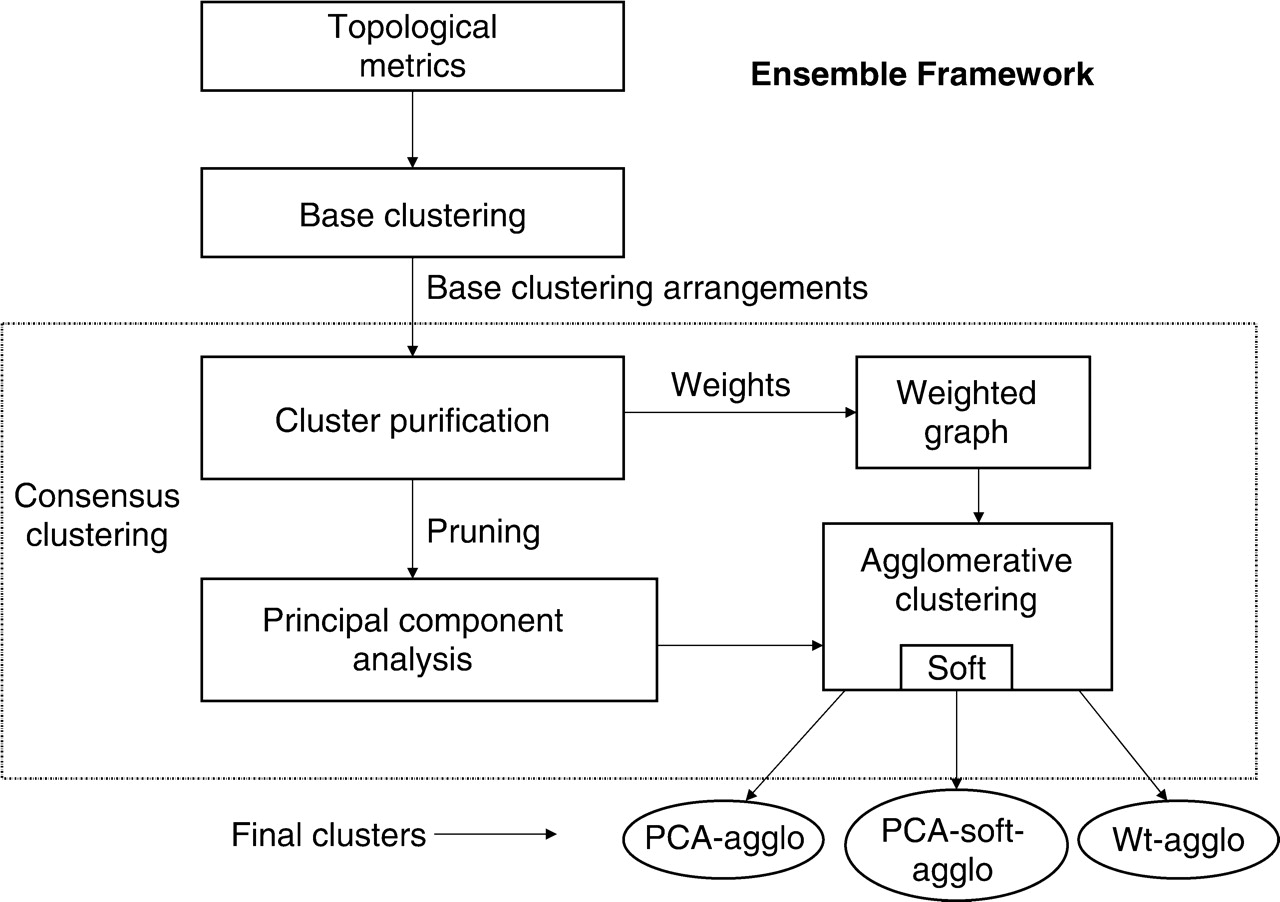
\includegraphics[scale=0.3]{./ensemble_cluster.jpeg}
\caption{Ensemble Framework for Clustering}
\label{fig:ensemble_cluster}
\end{figure}

In Figure \ref{fig:ensemble_cluster}, a flow for the ensemble framework can be seen. In  this figure 
there are two topological similarity metrics that will be used i.e., consensus methods 
and base clustering algorithms. The metrics are used to identify the reliability of PPI 
network interactions. Then based on that eliminate edges that give more false 
positives.\cite{wu_comprehensive_2020} The edge elimination is determined based on the 
weight assigned to edges and that weight is determined by topological features such as 
edge betweenness and clustering coefficient.

Initially, to obtain base clusters three conventional graph clustering algorithms are applied:
\begin{itemize}
    \item \textbf{Direct k-way partitioning} is a clustering solution in which $k$ objects are selected from the data set, these objects act as seed for the $k$ clusters. They are then assigned to each cluster based on the how much similar they are to these clusters. This is continuously refined so that the I2 clustering criterion function could be optimized.
    \item \textbf{Multilevel k-way partitioning} works in three phases, which are coarsening, initial partitioning and refinement. In coarsening, the original graph is divided into smaller graphs. Then in the next phase k-way partitioning of the coarsest graph takes place which satisfies the balance constraints and minimizes the cut value. Allowing for the partitioning to be projected back to the original graph. Finally, refinement reduces the edge-cut while making sure that balance constraints are not affected.  
    \item \textbf{Repeated bisections} is a top-down clustering solution, in which input matrix is clustered into two groups. After that, one of the groups is selected and bisected until the desired number of clusters are found. The clusters are bisected at each point to optimize the I2 clustering criterion function.
\end{itemize}

After getting the base clusters, the next step would be to combine the clusters to get a consensus clustering. To do that, we have to apply a consensus technique which consists of three stages:

\begin{itemize}
    \item \textbf{Cluster Purification}, the objective here is to find clusters that are less consistent with the topology of the original graph. To do that, a reliability measure for each cluster is defined which is based on the topology of proteins in the cluster. Then an intra-cluster distance, i.e., the average shortest path distance between all pair of proteins, is measured for each cluster. The reliability of a cluster is inversely proportional to its intra-cluster distance. A threshold value is then set to prune away weak clusters.
    \item \textbf{Dimensionality Reduction}: Even after pruning, the remaining clusters would still be a lot and the scaling of these clusters to higher dimensional points would likely prove to be inefficient. Which is why the dimensionality reduction would reduce the number of dimensions of cluster-membership matrix without affecting the information needed for clustering. Here, a logistic Principal Component Analysis (PCA) would be used to reduce the dimensions. After this, traditional clustering algorithms can be applied here to get the consensus clustering arrangements. 
    \item In \textbf{Consensus clustering} two consensus clustering algorithms would be applied on the PCA representation obtained from the previous step. The first algorithm, Recursive Bisection algorithm, performs the best of the three base algorithms. Then Agglomerative Hierarchical algorithm, a bottom-up clustering algorithm, assigns each object to its own cluster then continuously merge the pair of clusters until a single or desired number of clusters are obtained.  
\end{itemize}

Now on the acquired clusters there could be a possibility that some proteins are multi-functional. So to account for such cases \textsc{soft consensus clustering} would be applied in the agglomerative hierachical algorithm as there can be some proteins that are part of different clusters.

\chapter{Software Requirement Specification (SRS)}
\label{chap:srs}

\section{Functional Requirements}

We have to develop various pieces of code to materalize this project that ranges from collecting data to representing PPIN as networks using libraries such \texttt{Networkx, iGraph, Numpy, Matplotlib, Pandas} to running large analysis algorithms through the help of various libraries such as \texttt{Tensorflow, Scikit-Learn}. 

Furthermore, we will implement our own classes and methods in \texttt{Python} that will serve various purposes and and will work in-tandem. These will be comprised of wrapping the above mentioned libraries and their methods, and other other open source bioinformatics libraries such as PyBioMed \cite{dong_pybiomed_2018}. A functional hierarchy of all of our final work may look like:
\begin{outline}
  \1 \texttt{Data API}
%   \2 Function 1:
%   \2 Function 2:
  \1 \texttt{PPIN Class}
%   \2 Function 1:
%   \2 Function 2:
  \1 \texttt{Analysis Class}
  \1 \texttt{Prediction Class}
  \1 \texttt{Visualization API}
\end{outline}

% --- The above is to be modified as per your project, e.g. a flat list if your system has limited functional requirements.

% \section{Non-functional Requirements}

% This sections mentions the specific non-functional requirements of our system. These generally address performance, scalability, safety, availability, deployment etc.


\section{External Interfaces}

\subsection{Visualization}
To visualize the protein-protein interactions (PPI), we will potentially be using a software, like PyMol. PyMol is a 3D protein visualizer software that can visualize single proteins and could also used to show the PPI. Figure 3.1 shows a 3D protein-ligand interaction that we did manually to depict what our potential final deliverable would look like. The input for the protein files would in the form of a Protein Data Bank (PDB) ID. We would get these files as a result of the protein clusters that we get from the clustering algorithms from the ensemble framework.
\begin{figure}[h!]
\centering
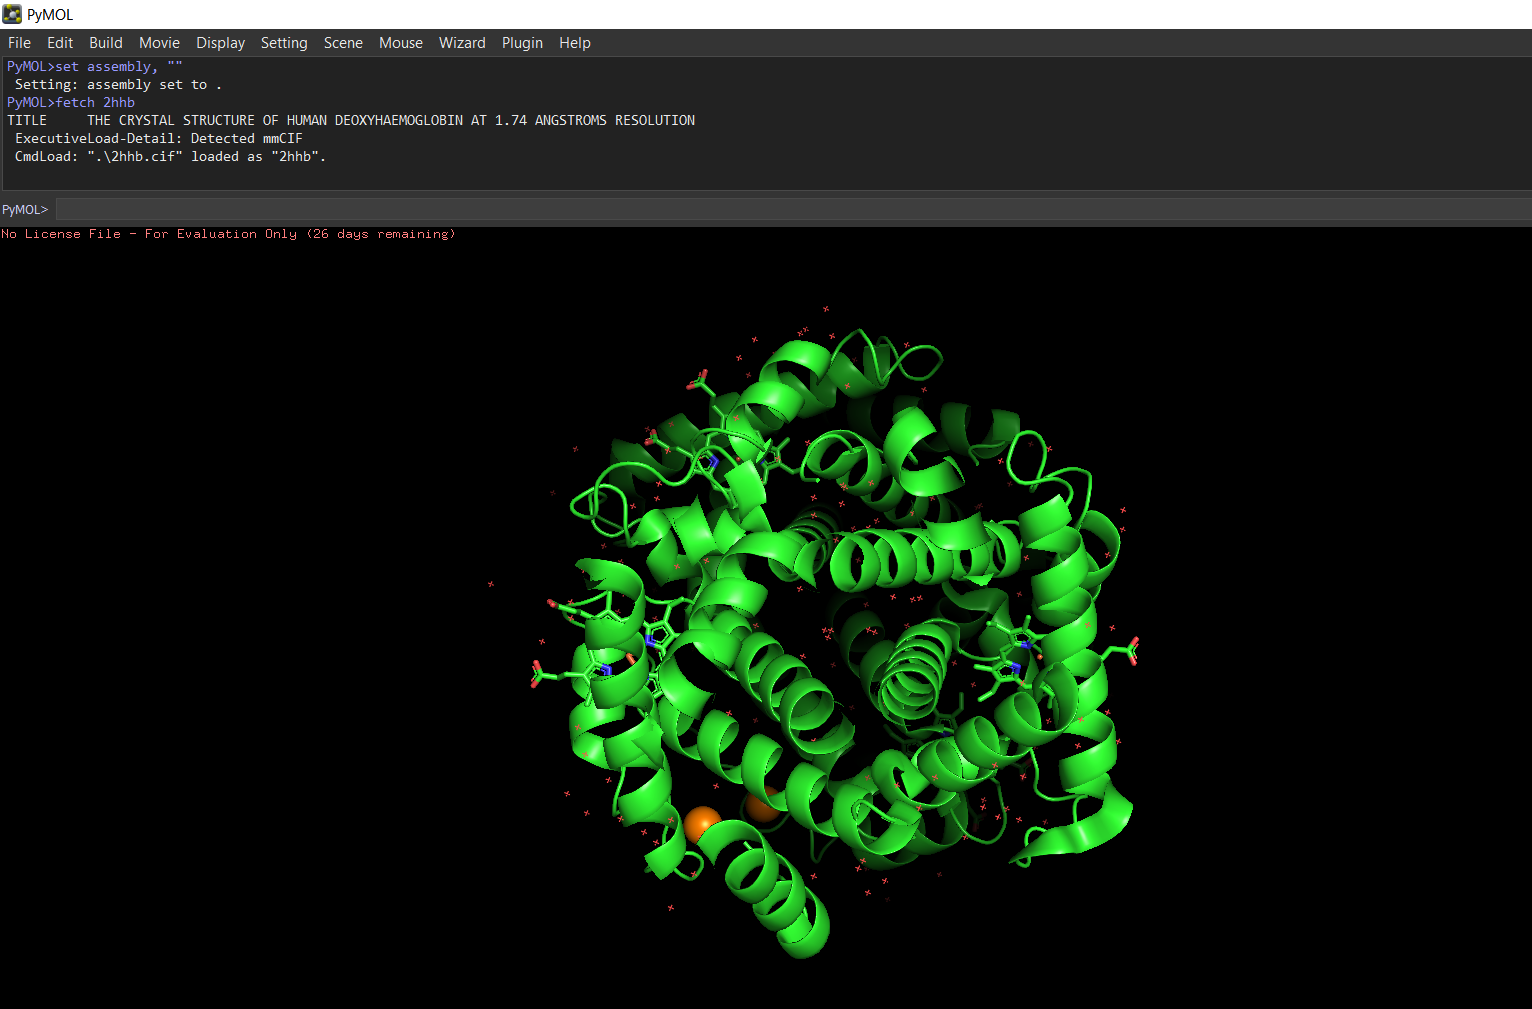
\includegraphics[scale=0.5]{./PyMol.png}
\caption{Protein-Ligand Interaction}
\label{fig:PyMol}
\end{figure}

\section{Datasets}
% This section describes the specific dataset(s) used to build our system. An appropriate snapshot of the dataset(s) is also included. Futher details, when needed, are presented in the appendix.
The collection and compilation of datasets to form a complete database of protein-protein interaction networks (PPIN) is an integral part of the project. The datasets used in our project are centered around one singular species; \textit{homo sapiens}, without any restriction on the list of proteins forming the global network. The datasets are extracted from online repositories such as BioGRID, APID, STRING that collect data about protein protein interactions from biological and bio-informatic literature. 

% \subsection{Purpose}

\subsection{PPIN Datasets}
The PPIN datasets that the project will work with will be from a singular species; \textit{homo sapiens}, as mentioned earlier and will be extracted from multiple online repositories. The data preserved in these datasets will be in a pairwise format where each row stores information such as the \textit{uniProtKB} and name of each protein in a protein-protein interaction pair, along with the MINT score of the interaction.\\\\
The information for each column entry in the dataset is as follows:
\begin{itemize}
    \item \textbf{UniProtKB ID:} The uniProtKB of a protein is the unique primary identifier of an interactor stored in the uniProt database. It is an ID assigned to a protein interactor for identification within uniProt and is considered universal.\\
    There will be two columns of UniProt IDs(UniProtA and UniProtB), one for each protein interactor (in this case protein A and protein B) in a protein-protein interaction pair.
    \item \textbf{Gene Name:} The recommended name used to officially represent any gene, adhering to the gene nomenclature.\\
    There will be two columns of Gene Names (GeneName A and GeneName B), one for each protein interactor (in this case protein A and protein B) in a protein-protein interaction pair.
    \item \textbf{Score:} The score assigned to any interaction pair is a value between 0 and 1 that is representative of all the cumulative experimental evidence of an existing interaction between the two interactors, as retrieved from multiple different databases. The score is calculated by using the MINT scoring function given as follows:
    $$S = 1-a^{-x}$$
    where, $a$ represents the initial slope of the curve and is arbitrarily chosen and $x$ represents the combined experimental evidence, and is obtained by summing up experimental evidence weighted by coefficients $d$ and $e$, which cater to the size of the experiment and method of experimentation respectively. $x$ can be given as follows:
    $$x = \sum_{i}d_{i}e{i} + \frac{n}{10}$$
    In the function above, $n$ represents the number of publications that give supporting evidence for existence of the interaction.
    The MINT score ensures that only those interactions supported by multiple experimental techniques and publications have a score close to 1 and those that lack sufficient evidence have a lower score. 
\end{itemize}


% \subsection{Protein Data}
\subsection{Table of Datasets}
The list of sources or online repositories from which the data will be extracted is given as follows:
\begin{table}[htpb]
      \centering
      \caption{A list of PPI databases.}
      \vspace{1 em}
      \label{tab:dataset1}
      \begin{tabular}{l|l}
      \hline
      Name & Website \\
      \hline
      DIP & \url{http://dip.doe-mbi.ucla.edu/dip/Main.cgi}\\
      BioGRID & \url{https://thebiogrid.org/} \\
      APID & \url{http://cicblade.dep.usal.es:8080/APID/init.action}\\
      HPRD & \url{http://www.hprd.org/} \\ 
      MINT & \url{https://mint.bio.uniroma2.it}\\
    STRING & \url{https://string-db.org/} \\
    \hline
    \end{tabular}
  \end{table}

\subsection{Method for Compilation}
The acquisition of datasets and compilation of the datasets is an integral part of the formation of a usable database. The datasets will firstly be collected by running a query on the online repositories which extracts all possible PPIN for human proteins such as GRB2.\\\\The key challenge then presents itself in the form of the compilation of the datasets, where each extracted and downloaded dataset is in a different format in terms of how the data is presented as well as the type of data that is presented. Some data does not have the MINT score included which can then be confirmed by running a query on the MINT repository or on MENTHA.\\\\
The datasets are first be converted into a standardized readable format, preferably in the form of a TSV. The data within will then be standardized in terms of the presentation of the data. The standardized datasets will then be compiled and filtered to remove incomplete or multiple instances of the data. The steps are highlighted in the compilation pipeline given in the diagram below.
\begin{figure}[h!]
    \centering
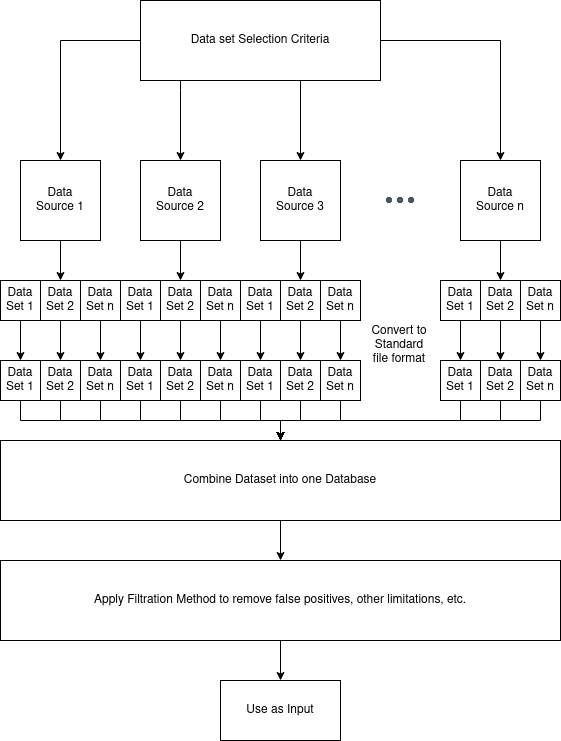
\includegraphics[scale=0.7]{Final-Report-Kavish-1/dataset-comp.png}
\caption{Database Compilation Pipeline.}
\label{fig: data_pipelinediag}
\end{figure}


% \begin{enumerate}
%     \item The online repositories will be queried for human proteins such as GRB2
%     \item The datasets will be downloaded and converted into TSV format
%     \item 
% \end{enumerate}
% \subsection{Interfacing with Dataset}

% \section{System Diagram}
% This diagram gives a high-level view of the different components of our system and the interactions between them. Each component and the particular tools/technologies/libraries used to build it are described.
% \begin{center}
    
% \begin{sidewaysfigure}

% \end{center}
% \end{sidewaysfigure}

% \chapter{Software Design Specification (SDS)}
% \label{chap:sds}
% This chapter presents an overview of our proposed architecture represented through a diagram. We also present the experimental design and the evaluation metrics that we will employ to evaluate the performance of our method. The information presented below is tentative and can be subject to change if a better approach is identified/discovered along the course of the project.

\section{Architecture Design}
\subsection{Proposed System Model}
The proposed system model will begin with the assumption that the data has been 
processed and filtered so as to reduce the noise within the data and process it 
according to the database compilation pipeline in Figure~\ref{fig: data_pipelinediag}. The dataset will contain the IDs and gene names of the proteins 
in each protein pair as well as their interaction score. This will then be used to 
create a PPI network object that can then be used in N base clustering algorithms to 
generate clusters. 

These base clustering algorithms will include the Direct k-way 
partitioning and multilevel k-level partitioning as described in Section~\ref{sec: 
ensemble framework}. After obtaining clusters we will then proceed to the core of the
ensemble framework. We will purify these clusters, prune them and apply principle component analysis (PCA) on the clusters. The clusters will also be turned into weighted graphs by adding weights after the purification block. The weighted graphs and the PCA together will then be used for agglomerate clustering which will give us out final cluster outputs which will be tested against our evaluation metrics.

A high level representation of the proposed system model can be seen in Figure~\ref{fig: systemdiag}.
\begin{figure}[h!]
    \centering
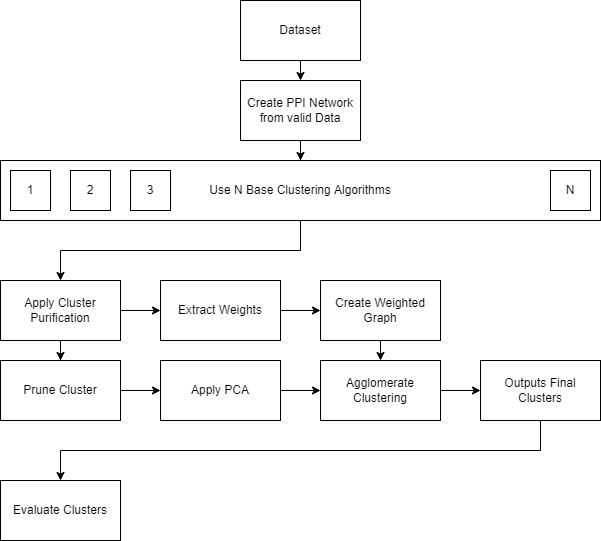
\includegraphics[scale=0.7]{Documentation/Final-Report-Kavish-1/system_diagram1.png}
\caption{Proposed System Diagram}
\label{fig: systemdiag}
\end{figure}

% \begin{enumerate}
% \item{Hypothesis}
% \item{Method}
% \item{Results}
% \item{Limitations of Methodology}
% \end{enumerate}

\section{Experimental Design \& Evaluation Metrics}
Since the problem of identifying protein complexes essentially boils down to a classification 
problem, where we are identifying known protein complexes (subgraphs) from a sea of candidate 
subgraphs. Therefore, after we obtain our final result, we can use a testing set generated from 
preexisting protein complex databases to evaluate our result. We will use the evaluation metrics 
that are generally used for classification problems. These include: 
\begin{enumerate}
\item{Precision \& Recall}: Precision is the fraction of relevant complexes among identified complexes while recall is the fraction of relevant complexes that were identified. Mathematically, they are computed as:
\[\text{Precision } = \frac{\{p \; | \; p \in P \; \wedge \; \exists r \in R, p \text{ matches } r\}}{|P|}\]
\[\text{Recall } = \frac{\{r \; | \; r \in R \; \land \; \exists p \in P, \; r \text{ matches } p\}}{|R|}\]

\item{$F$-Measure}:
The $F$-measure or $F$-score is calculated using precision and recall. More specifically, we will use the $F_1$ 
score to evaluate the performance of our method. The $F_1$ score is the harmonic mean of precision and recall and is given as:

\[F \text{ measure } = \frac{2 \cdot \text{Precision} \cdot \text{Recall}}{\text{Precision } + \text{ Recall}}\]

\item{Confusion Matrix}: We can create a confusion matrix $T$ from $n$ reference protein complexes and $m$ identified clusters:
\[T = \begin{bmatrix}
t_{1,1} & \ldots & t_{1,m} \\ 
\vdots & \ddots & \vdots \\ 
t_{1,n} & \ldots & t_{n,m}  
\end{bmatrix}\]
where $t_{i,j}$ indicates the number of proteins that the $i$-th known protein complex and the 
$j$-th cluster have in common. Using the confusion matrix, we can generate three other useful metrics:
\begin{itemize}
    \item Sensitivity (Sn) can be computed as:
    \[\text{Sn } = \frac{\sum_{i=1}^n \max_j{t_{ij}}}{f}\]
    \item Positive Predictive Value (PPV) is given as:
    \[\text{PPV } = \frac{\sum_{j=1}^m \max_i{t_{ij}}}{\sum_{j=1}^m \; \sum_{i=1}^n t_{ij}}\]
    \item Accuracy (Acc) can be computed using:
    \[\text{Acc } = \sqrt{\text{Sn} \times \text{PPV}}\]
\end{itemize}
\end{enumerate}


% \chapter{Experiments and Results}
% \label{chap:results}
% We did many experiments and got the best results.

% \chapter{Conclusion and Future Work}
% \label{chap:outro}
% Our work is awesome. We would write more but we need to catch the flight to collect our Turing Award.

% \begin{appendices}

% \titleformat{\chapter}[hang]{\bf\huge}{Appendix \thechapter.}{2pc}{}
  
% % This appendix is optional.
% \chapter{More Math}
% Here, we describe the background math for the techniques used in the text.

% % This appendix is required if the data set is not fully described in the main text.
% \chapter{Data}
% Here is a dump of our 2TB data set. Enjoy!

% % This appendix is required if the code is not fully described in the main text.
% \chapter{Code}
% % EITHER dump your code here. No one except HEC likes this.
Here is our code.

% inspired by https://xkcd.com/221/
\begin{lstlisting}[language=python, showstringspaces=false,frame=single]
  print('Hello World!')
  print('Computing true random number.')
  print('Capturing interstellar radiation.')
  print('This will take time!')
  import random
  import time
  time.sleep(3600*random.randint(1,10))
  print(4)
\end{lstlisting}

% OR, link to your GitHub repository. Everyone but HEC will like this.
Our code can be found at \url{https://github.com/habib-university/Kaavish-Template}.

%%% Local Variables:
%%% mode: latex
%%% TeX-master: "../report"
%%% End:

% \end{appendices}

% % Print the bibliography with a ToC entry and titled, "References".
\chapter{Software Design Specifications (SDS)}
\label{chap:sds}
This chapter presents an overview of our proposed architecture represented through a diagram. We also present the experimental design and the evaluation metrics that we will employ to evaluate the performance of our method. The information presented below is tentative and can be subject to change if a better approach is identified/discovered along the course of the project.

\section{Architecture Design}
\subsection{Proposed System Model}
The proposed system model will begin with the assumption that the data has been 
processed and filtered so as to reduce the noise within the data and process it 
according to the database compilation pipeline in Figure~\ref{fig: data_pipelinediag}. The dataset will contain the IDs and gene names of the proteins 
in each protein pair as well as their interaction score. This will then be used to 
create a PPI network object that can then be used in N base clustering algorithms to 
generate clusters. 

These base clustering algorithms will include the Direct k-way 
partitioning and multilevel k-level partitioning as described in Section~\ref{sec: 
ensemble framework}. After obtaining clusters we will then proceed to the core of the
ensemble framework. We will purify these clusters, prune them and apply principle component analysis (PCA) on the clusters. The clusters will also be turned into weighted graphs by adding weights after the purification block. The weighted graphs and the PCA together will then be used for agglomerate clustering which will give us out final cluster outputs which will be tested against our evaluation metrics.

A high level representation of the proposed system model can be seen in Figure~\ref{fig: systemdiag}.
\begin{figure}[h!]
    \centering
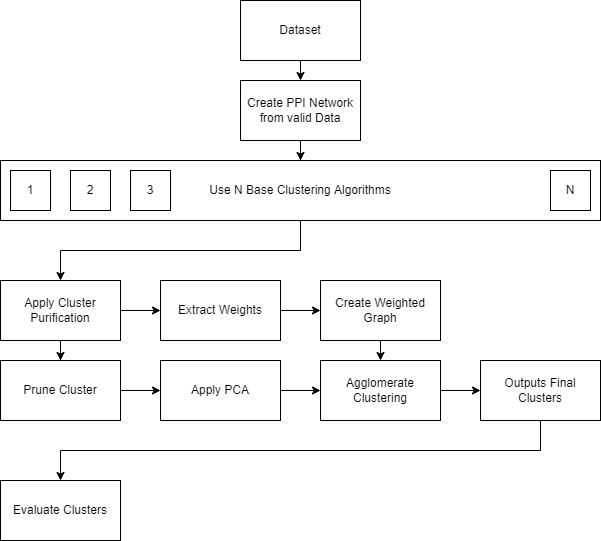
\includegraphics[scale=0.7]{Documentation/Final-Report-Kavish-1/system_diagram1.png}
\caption{Proposed System Diagram}
\label{fig: systemdiag}
\end{figure}

% \begin{enumerate}
% \item{Hypothesis}
% \item{Method}
% \item{Results}
% \item{Limitations of Methodology}
% \end{enumerate}

\section{Experimental Design \& Evaluation Metrics}
Since the problem of identifying protein complexes essentially boils down to a classification 
problem, where we are identifying known protein complexes (subgraphs) from a sea of candidate 
subgraphs. Therefore, after we obtain our final result, we can use a testing set generated from 
preexisting protein complex databases to evaluate our result. We will use the evaluation metrics 
that are generally used for classification problems. These include: 
\begin{enumerate}
\item{Precision \& Recall}: Precision is the fraction of relevant complexes among identified complexes while recall is the fraction of relevant complexes that were identified. Mathematically, they are computed as:
\[\text{Precision } = \frac{\{p \; | \; p \in P \; \wedge \; \exists r \in R, p \text{ matches } r\}}{|P|}\]
\[\text{Recall } = \frac{\{r \; | \; r \in R \; \land \; \exists p \in P, \; r \text{ matches } p\}}{|R|}\]

\item{$F$-Measure}:
The $F$-measure or $F$-score is calculated using precision and recall. More specifically, we will use the $F_1$ 
score to evaluate the performance of our method. The $F_1$ score is the harmonic mean of precision and recall and is given as:

\[F \text{ measure } = \frac{2 \cdot \text{Precision} \cdot \text{Recall}}{\text{Precision } + \text{ Recall}}\]

\item{Confusion Matrix}: We can create a confusion matrix $T$ from $n$ reference protein complexes and $m$ identified clusters:
\[T = \begin{bmatrix}
t_{1,1} & \ldots & t_{1,m} \\ 
\vdots & \ddots & \vdots \\ 
t_{1,n} & \ldots & t_{n,m}  
\end{bmatrix}\]
where $t_{i,j}$ indicates the number of proteins that the $i$-th known protein complex and the 
$j$-th cluster have in common. Using the confusion matrix, we can generate three other useful metrics:
\begin{itemize}
    \item Sensitivity (Sn) can be computed as:
    \[\text{Sn } = \frac{\sum_{i=1}^n \max_j{t_{ij}}}{f}\]
    \item Positive Predictive Value (PPV) is given as:
    \[\text{PPV } = \frac{\sum_{j=1}^m \max_i{t_{ij}}}{\sum_{j=1}^m \; \sum_{i=1}^n t_{ij}}\]
    \item Accuracy (Acc) can be computed using:
    \[\text{Acc } = \sqrt{\text{Sn} \times \text{PPV}}\]
\end{itemize}
\end{enumerate}



\printbibliography[heading=bibintoc,title={References}]

\end{document}

%%% Local Variables:
%%% mode: latex
%%% TeX-master: t
%%% End:
